\documentclass[aspectratio=169,t,13pt,usenames,dvipsnames]{beamer}
\usetheme[lily]{PaloAlto}
\usecolortheme{dolphin}
\usepackage{tikz}
\usepackage{adjustbox}
\usetikzlibrary{quantikz}
\usepackage{xcolor}
\logo{
\includegraphics[height=2cm]{logo.pdf}}
\def\ColorR#1{\textcolor{BrickRed}{#1}}
\def\ColorG#1{\textcolor{OliveGreen}{#1}}
\def\ColorB#1{\textcolor{NavyBlue}{#1}}
\definecolor{links}{HTML}{2E8B57}
\hypersetup{colorlinks,linkcolor=,urlcolor=links}
\def\LinkArrow#1{%
\mbox{$\,$\href{#1}{\mbox{\vrule width 0pt height 0ex depth 0pt$\mapsto$}}}$\,$}
\def\True{\mbox{\texttt{True}}}
\def\False{\mbox{\texttt{False}}}
\def\Zero{\mbox{$0$}}
\def\One{\mbox{$1$}}
\def\Not#1{%
\ensuremath{\Overline{#1}}}
\def\Xor#1#2{\ensuremath{#1\oplus #2}}
\def\Nand#1#2{%
\ensuremath{\mbox{Nand}(#1,#2)}}
\def\And#1#2{%
\ensuremath{#1 \wedge #2}}
\def\Or#1#2{%
\ensuremath{#1 \vee #2}}
\def\Conj#1{%
\ensuremath{#1^{\star}}}
\def\Mag#1{%
\ensuremath{|\,#1\,|}}


\def\BigSkip{%

\bigskip

}

\def\MedSkip{%

\medskip

}
\def\SmallSkip{%

\smallskip

}
\newcommand{\tolstrut}{%
  \vrule height\dimexpr\fontcharht\font`\A+.1ex\relax width 0pt\relax
}

\DeclareRobustCommand{\Overline}[1]{%
  \ensuremath{\overline{\raisebox{0pt}[1.2\height]{#1}}}%
}
\newenvironment{TIKZP}[1][scale=1.0]{%
\adjustbox{valign=t}\bgroup
\begin{tikzpicture}[#1]
}{%
\end{tikzpicture}
\egroup
}

\long\def\TwoUnequalColumns#1#2#3#4{%
\begin{columns}
\begin{column}{#1}
#3
\end{column}
\begin{column}{#2}
#4
\end{column}
\end{columns}
}
\long\def\TwoColumns#1#2{%
\TwoUnequalColumns{0.5\textwidth}{0.5\textwidth}{#1}{#2}%
}
\long\def\OnlyRemark#1#2{%
\only<#1>{\Remark{#2}}}

\long\def\Remark#1{%
\begin{block}{Remark}
#1
\end{block}}
\long\def\Example#1{%
\begin{example} #1\end{example}}
\def\VV{\textit{vice versa}}
\def\QZero{\ket{0}}
\def\QOne{\ket{1}}
\def\TZPoint#1#2#3{%
\draw[fill=black] (#1) circle (2pt) node[#3] {#2} ;}
\def\UnitComplexCircle{%
\draw [<->] (-1.5, 0) -- (1.5, 0)  node[right] {$\Re{}$} ;
   \draw [<->] (0,-1.5) -- (0, 1.5) node[above] {$\Im{}$} ;

   \draw (0, 0) circle (1) ;
   }
\def\TZText#1#2#3{%
  \draw (#1) node [#3] {#2};
}
\def\Exp#1{\ensuremath{e^{#1}}}
\def\Polar#1#2{\ensuremath{#1\hbox to 0.1pt{\hss}\Exp{i\relax#2}}}
%%
%% #1 -- lower left x
%% #2 -- lower left y
%% #3 -- upper right x
%% #4 -- upper right y
%% #5 -- num lines
\def\PFilter#1#2#3#4#5{

    \draw (#1,#2) -- (#3,#2) -- (#3,#4) -- (#1,#4) -- cycle;
    \foreach \i in {1,...,#5}
    {
        \pgfmathsetmacro{\PFilterInc}{#1 + (#3-#1) / #5 * \i}
        % \edef\PFilterInc{\pgfmathresult}
        \draw (\PFilterInc, #2) -- (\PFilterInc, #4);
    }
}
\def\Vskip#1{\mbox{}\vskip #1\mbox{}}
\def\Hskip#1{\mbox{}\hskip #1\mbox{}}
\author{Ron K.~Cytron}
\institute{Washington University\\Saint Louis, Missouri}
\setbeamertemplate{footline}[frame number]
%% #1 -- lecture number
%% #2 -- lecture title
%% #3 -- lecture subtitle
%% #4 -- lecture label
\def\SetTitle#1#2#3#4{%
   \lecture[#1]{#2}{lec:#4}%
   \title{#2}%
   \subtitle{#3}%
   \date{\today}%
   \begin{frame}\maketitle\end{frame}%
}
\def\Kaye{\href{https://dl.acm.org/doi/10.5555/1206629}{Kaye}}
\def\MikeIke{\href{https://dl.acm.org/doi/10.5555/1972505}{Nielson~and~Chuang}}

%% #1 -- options
%% #2 -- width
%% #3 -- height
%% #4 -- signals
\newenvironment{GateBox}[4][scale=1.0]{%
\edef\Signals{#4}
\edef\Height{#3}
\edef\Width{#2}
\pgfmathsetmacro{\Max}{\Signals}
\pgfmathsetmacro{\Vsep}{\Height / \Max}
\pgfmathsetmacro{\Wlen}{\Width / 5}
\def\CalcY##1{%
0}
\def\Input##1##2{%
   \pgfmathsetmacro{\Xone}{-\Wlen}
   \pgfmathsetmacro{\Xtwo}{0}
   \pgfmathsetmacro{\MyY}{\Height - 0.5 * \Vsep - ##1*\Vsep}
   \draw[->] (\Xone,\MyY) node[left] {##2} -- (\Xtwo,\MyY);
}
\def\Output##1##2{%
   \pgfmathsetmacro{\Xone}{\Width}
   \pgfmathsetmacro{\Xtwo}{\Width + \Wlen}
   \pgfmathsetmacro{\MyY}{\Height - 0.5 * \Vsep - ##1*\Vsep}
   \draw[->] (\Xone,\MyY) -- (\Xtwo,\MyY) node[right] {##2};
}
\def\BoxLabel##1{%
\node[draw, fit={(0,0) (\Width,\Height)}, inner sep=0pt, label=center:##1] (A) {};
}
\begin{TIKZP}[#1]
   \draw (0,0) rectangle(#2,#3);
}{%
\end{TIKZP}
}


\begin{document}
\SetTitle{2}{Reversible Computations}{No energy lost or gained}{reverse}

\begin{frame}{Overview}
\begin{itemize}
    \item Quantum computations involve gates that are \emph{unitary} and therefore are invertible.
    \item Quantum computations are delicate and noise must be kept to a minimum.  Interactions with the environment will cause the quantum system to collapse (\href{https://en.wikipedia.org/wiki/Quantum_decoherence}{decoherence}).
    \item We study a mechanical computer first where it is clear that a nonreversible computation gains or loses energy.
    \item We can build reversible circuits for classical and quantum computations.
    
\end{itemize}
\end{frame}

\begin{frame}{The \href{https://en.wikipedia.org/wiki/Billiard-ball_computer}{billiard ball computer}}{When a single ball enters at a time}
\TwoColumns{%
Consider the mechanical \emph{and} gate shown here.
\begin{itemize}
    \item<1-> A ball entering from the top
    \only<2->{will emerge from the ``1-out'' hole.}
    \item<3-> A ball entering from the left
    \only<4->{will emerge from the ``0-out'' hole.}
    
\end{itemize}
}{%

\begin{TIKZP}
\node at (0,0)
    {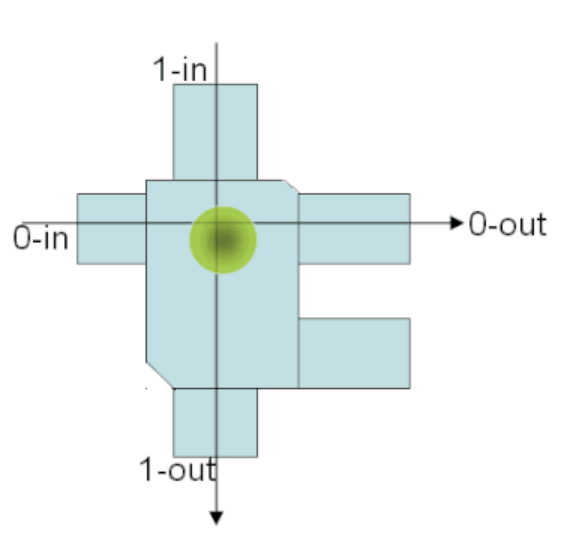
\includegraphics[width=0.7\textwidth]{2/single.png}};
\visible<1>{\fill[color=SpringGreen] (-.59,2.2) circle(0.25);}
\visible<2>{\fill[color=SpringGreen] (-.59,-2.1) circle(0.25);}
\visible<3>{\fill[color=SpringGreen] (-2.7,0.3) circle(0.25);}
\visible<4>{\fill[color=SpringGreen] (2.5,0.3) circle(0.25);}
\end{TIKZP}

}
\only<5->{
\MedSkip{}No energy is put in or taken out of the system.  The ball has its own energy, maintained throughout its motion through the box.}
    
\end{frame}
\begin{frame}{The billiard ball computer}{When two balls enter simultaneously}
\TwoUnequalColumns{0.6\textwidth}{0.4\textwidth}{%
Here, two balls enter, one from the top, and one from the left
\begin{itemize}
    \item<1-> A ball entering from the top and a ball entering from the left at the same time
    \only<2->{will \alert<2>{collide here}.}
    \item<3-> They bounce internally at the same time.
    \item<4-> One ball emerges from the ``AND-output'' chute and the other emerges from the ``1-out'' chute.
    
\end{itemize}
}{%
\Vskip{-3.2em}\Hskip{-0em}
\begin{TIKZP}
\node at (0,0)
    {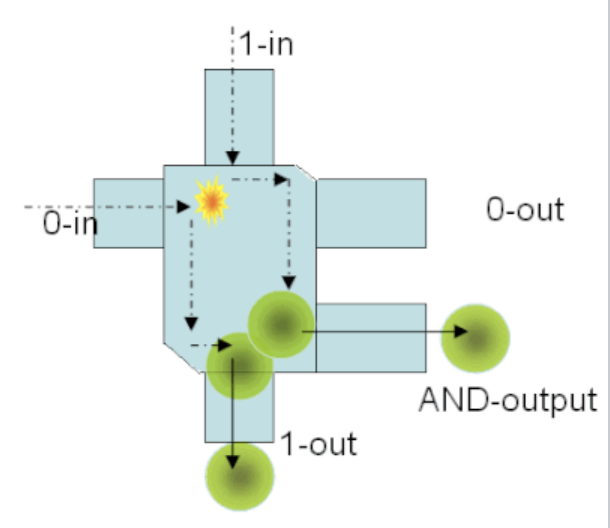
\includegraphics[width=0.7\textwidth]{2/double.png}};
\visible<1>{\fill[color=SpringGreen] (-.45,1.8) circle(0.25);}
\visible<2>{\fill[color=red] (-.6,0.4) circle(0.25);}
\visible<1>{\fill[color=SpringGreen] (-2.2,0.3) circle(0.25);}
\end{TIKZP}

}
\only<5->{
\SmallSkip{}Again, the energy of the box remains the same throughout.\Remark{It would take energy to \emph{stop} the ball from exiting the ``1-out'' chute.}}

    
\end{frame}

\section{Reversible gates}
\begin{frame}{Not and And}{From page 12 of \Kaye{}.}
\TwoColumns{%
\begin{itemize}
    \item<1-> The \emph{not} gate is reversible and is in fact its own inverse.
    \item<2-> Is \And{a}{b} reversible if we know $a$?  \only<3->{No.} \only<3>{If $a=0$, $b$ could be either $0$ or $1$.}
    \item<4-> We need a copy of both inputs to create a reversible \emph{and} gate.
\end{itemize}
 
}{%


\begin{center}
\only<1>{
\begin{GateBox}[scale=0.5]{2}{1}{1}
\BoxLabel{Not}
\Input{0}{$a$}
\Output{0}{\Overline{a}}
\end{GateBox}}

\only<2-3>{\begin{GateBox}{2.5}{1}{2}
\BoxLabel{Copy $a$/And}
\Input{0}{$a$}
\Input{1}{$b$}
\Output{0}{$a$}
\Output{1}{\And{a}{b}}
\end{GateBox}}


\only<4>{\begin{GateBox}{2.5}{1}{3}
\BoxLabel{Reversible?}
\Input{0}{$a$}
\Input{1}{$b$}
\Output{0}{$a$}
\Output{1}{$b$}
\Output{2}{\And{a}{b}}
\end{GateBox}}

\only<5>{\begin{GateBox}{2.5}{1.5}{3}
\BoxLabel{\mbox{\stackbox[c]{Reversible\\ And}}}
\Input{0}{$a$}
\Input{1}{$b$}
\Input{2}{\Zero{}}
\Output{0}{$a$}
\Output{1}{$b$}
\Output{2}{\And{a}{b}}
\end{GateBox}}
\end{center}
}
\MedSkip{}
   \only<4>{
    However, this box must generate energy to produce the third output.  To conserve energy, a reversible box must have the same number of inputs as outputs.}

\only<5>{This box enables reversal of the computation and it accepts an \href{https://en.wikipedia.org/wiki/Ancilla_bit}{ancilla} bit as a third input.}

\OnlyRemark{5}{The circuit elements involved in quantum computations must be \emph{reversible} and must contain the same number of inputs as outputs.}
\end{frame}

\begin{frame}{The Toffoli / CCNOT gate}{Uses the third input to greater advantage}
\TwoColumns{%
\begin{itemize}
    \item<1-> The signals $a$ and $b$ are copied to their respective outputs.
    \item<2-> The bottom output is computed as: 
    \only<2->{
    \Vskip{-2em}\begin{description}
        \item[$c=0$] The output is \And{a}{b}.
        \item[$c=1$] The output is \Nand{a}{b}.
    \end{description}}
    \item<2-> Because it can realize Nand, this reversible gate is \emph{universal} for constructing classical circuits.
    \item<3-> The gate is known in quantum computing as the \href{https://en.wikipedia.org/wiki/Toffoli_gate}{Tofolli Gate}.
\end{itemize}
}{%
\begin{center}
\begin{GateBox}{2.5}{1.5}{3}
\only<1-2>{\BoxLabel{\mbox{f(a,b)=\And{a}{b}}}}
\only<3-4>{\BoxLabel{Tofolli Gate}}
\only<5->{\BoxLabel{\mbox{\stackbox[c]{Tofolli Gate\\ CCNOT}}}}

\Input{0}{$a$}
\Input{1}{$b$}
\Input{2}{$c$}
\Output{0}{$a$}
\Output{1}{$b$}
\only<1-3>{\Output{2}{\Xor{c}{(\And{a}{b})}}}
\only<4->{\Output{2}{\Xor{(\And{a}{b})}{c}}}
\end{GateBox}
\end{center}
\only<4->{\MedSkip{}
An alternative view of this gate:
\begin{itemize}
    \item When $a$ and $b$ are both \True{}, the incoming signal $c$ is complemented on output.
    \item<5-> It is thus also called a controlled-controlled-Not gate, or CCNOT.
\end{itemize}
}
}
    
\end{frame}

\begin{frame}{Generally reversible computation}{From \Kaye{} page 14}
I need help with this
    
\end{frame}

\begin{frame}{CNOT gate}{Two-bit version of CCNOT}
\TwoColumns{%

\begin{itemize}
    \item $c$ controls whether the bottom output is a copy of $a$ or its complement.
    \item The computation is reversible because
    \[ \Xor{a}{(\Xor{c}{a})} = c \]
    so we can recover $c$.
\end{itemize}
}{%
\begin{GateBox}{2.5}{1.5}{2}
\BoxLabel{CNOT}

\Input{0}{$a$}
\Input{1}{$c$}
\Output{0}{$a$}
\Output{1}{\Xor{c}{a}}
\end{GateBox}
\begin{center}
\begin{tabular}{cc||cc}
\multicolumn{2}{c}{Inputs} &
\multicolumn{2}{c}{Outputs} \\
$a$ & $c$  & $a$ & \Xor{c}{a} \\ \hline
0 & 0 & 0 & 0 \\
0 & 1 & 0 & 1 \\
1 & 0 & 1 & 1 \\
1 & 1 & 1 & 0
\end{tabular}
\end{center}
}
    
\end{frame}
\end{document}